\documentclass[conference,a4paper]{IEEEtran}
% \IEEEoverridecommandlockouts % not needed here

% Core IEEE template packages
% Use natbib to support \citep/\citet used in the original content
\usepackage[numbers,sort&compress]{natbib}
\usepackage{amsmath,amssymb,amsfonts}
\usepackage{graphicx}
\usepackage{textcomp}
\usepackage{xcolor}

% Additional packages needed by the paper content (formatting only)
\usepackage{microtype}
\usepackage{booktabs}
\usepackage{siunitx}
% \usepackage{hyperref} % Removed for submission - no links allowed
\usepackage{cleveref}
\usepackage[utf8]{inputenc}
\usepackage[T1]{fontenc} % Better font encoding; reduces issues with accented/Unicode chars
\usepackage[top=1.9cm,bottom=2.65cm,left=2cm,right=2cm]{geometry} % Ensure minimum margins: top 1.9cm, bottom 2.53cm



% Increase column separation to meet 0.25 inch requirement
\setlength{\columnsep}{0.30in}

% (natbib provides \citep and \citet)

% Macros (unchanged)
\newcommand{\rmse}{\ensuremath{\mathrm{RMSE}}}
\newcommand{\rTwo}{\ensuremath{\mathrm{R}^2}}
\newcommand{\da}{\ensuremath{\mathrm{DA}}}

\begin{document}

\title{Benchmarking Transformers and Baselines for Multi-Horizon Stock Return Prediction with Technical and Earnings Features}

% \author{\IEEEauthorblockN{Nelson Siu}
% \IEEEauthorblockA{\textit{Division of Engineering Science}\\
% \textit{University of Toronto}\\
% Toronto, Canada\\
% \texttt{nelson.siu@mail.utoronto.ca}}}

% Minimal author block to satisfy IEEEtran class
\author{Nelson Siu \\
\textit{Division of Engineering Science} \\
\textit{University of Toronto} \\
nelson.siu@mail.utoronto.ca
\and
Jonathan H. Chan \\
\textit{Innovative Cognitive Computing} \\
\textit{King Mongkut's University of Technology Thonburi} \\
jonathan@sit.kmutt.ac.th}

\date{}

\maketitle

\begin{abstract}
We study daily multi-horizon stock return prediction on the Dow 30 ($h \in \{1,5,21\}$) using technical indicators and earnings features under a strict temporal split (train 2016--2019, val 2020, test 2021--2024). At $h{=}1$, LSTM attains the lowest RMSE (0.01622), narrowly ahead of GRU (0.01625), while Random Forest yields the highest DA (51.9\%). At $h{=}5$, Ridge achieves the best RMSE (0.03651). At $h{=}21$, LSTM delivers both the lowest RMSE (0.05084) and highest DA (55.0\%), edging TFT and GRU by 0.2--0.3\% RMSE and ~1 pp DA and outperforming tabular baselines by 31--38\% in RMSE. Adding earnings features increases DA by ~1 pp at $h{=}21$, and DA rises to 61.4\% within $\pm 3$-day earnings windows (vs. 53.9\% otherwise). By regime, GRU performs best in the 2022 bear (RMSE 0.0636) and LSTM in the 2023--2024 rally (RMSE 0.0475; DA 56.2\%). Overall, simple sequence models match or surpass TFT on this constrained daily panel, with tabular methods competitive at shorter horizons.
\end{abstract}

\section{Introduction}
Multi-horizon equity prediction remains challenging given noisy targets, regime dependence, and the potential for only small predictive signals. We present a clear, apples-to-apples comparison across model classes on the Dow 30 with realistic event sensitivity, evaluating how different modeling approaches perform under consistent data splits and feature sets.

\textbf{Contributions.}
\begin{itemize}
    \item \textit{Robust experimental design:} Strict temporal split with fixed Dow 30 constituents to mitigate survivorship bias.
    \item \textit{Model class comparison:} Direct comparison of sequence, transformer, and tabular models on identical feature sets.
    \item \textit{Comprehensive evaluation:} Multi-metric assessment across horizons with regime and earnings window analysis.
    \item \textit{Insights:} Identify model class advantages and explain why simpler models can rival complex ones on daily financial data.
\end{itemize}

\subsection{Hypotheses}

\textbf{H1 (Model class advantage).} Given multi-horizon forecasting with technical and earnings features on a pooled Dow 30 panel, the Temporal Fusion Transformer (TFT) will achieve lower \rmse{} and higher \da{} than strong baselines (LSTM, GRU, XGBoost, Random Forest, Ridge) on the 21-day horizon.

\textbf{H2 (Event features add value).} Adding earnings/event features to technical indicators will improve \da{} (and not worsen \rmse{}) relative to technical-only inputs at the 21-day horizon.

\textbf{H3 (Regime dependence).} Model rankings differ by market regime: sequence models (LSTM/GRU) will outperform tabular and transformer models during trending rally periods, while performance gaps will narrow or reverse during bear markets.

\paragraph{Decision criteria}
We evaluate each hypothesis using the held-out test set (see Abstract for split) across three random seeds:
\begin{itemize}
        \item \textit{H1:} TFT beats the best non-TFT model at $h{=}21$ by demonstrating either (i) a $\geq$2\,pp increase in \da{} or (ii) a $\geq$5\% relative improvement in \rmse{}, with non-overlapping 95\% bootstrap confidence intervals on the test set.
    \item \textit{H2:} Tech{+}Earnings vs Tech-only shows \da{} $\uparrow$ ($\geq$2\,pp) and \rmse{} does not increase (95\% CI overlap) for at least one strong model (e.g., TFT or XGBoost) at $h{=}21$.
  \item \textit{H3:} Best-in-class models differ across regimes (2022 bear vs 2023--24 rally), verified by per-regime leaderboards and non-overlapping bootstrap CIs.
\end{itemize}

\paragraph{Hypothesis rationale}
H1 assumes attention mechanisms handle long-term dependencies better \citep{lim2021temporal}. H2 follows from post-earnings-announcement drift \citep{bernard1989,schnaubelt2020}. H3 reflects the Adaptive Markets Hypothesis \citep{lo2004}. We set 2pp and 5\% thresholds to focus on practically meaningful differences.



\section{Related Work}
Approaches to multi-horizon financial forecasting (1-day, 1-week, 1-month) range from classical time series to modern ML, with mixed success across horizons and regimes.

\paragraph{Classical time-series baselines} ARIMA models remain standard but assume linearity and stationarity, limiting usefulness at longer horizons or during regime shifts \citep{box2015}. VAR shares these issues in high-dimensional, nonstationary settings. GARCH captures conditional variance rather than mean returns, restricting its role in multi-step prediction.

\paragraph{Traditional ML baselines and horizon effects} Tree ensembles and SVMs often outperform linear models with engineered features, but accuracy declines with horizon length due to error accumulation \citep{gu2018,chen2016xgboost}. Surveys confirm this degradation (e.g., 1-day to 20-day) across assets and markets \citep{zhang2023review}. In stock panels, ML methods surpass simple rules on cross-sectional tasks, though gains depend on validation design \citep{gu2018}.

\paragraph{Deep and hybrid architectures} RNNs (LSTM, GRU) capture temporal dependencies and often beat classical and tree models \citep{hochreiter1997long,cho2014learning,fischer2018,selvin2017}. Hybrids like CNN-LSTM improve short- and long-horizon forecasts by extracting local patterns first \citep{selvin2017}. Echo State Networks (ESN) offer efficient reservoir-based sequence modeling \citep{jaeger2001esn}.

\paragraph{Attention and transformers} Attention mechanisms highlight horizon-specific context; e.g., attention-based CNN-LSTMs for crypto \citep{xu2022bitcoin}. The Temporal Fusion Transformer (TFT) \citep{lim2021temporal} produces multi-horizon outputs via recurrent encoders, static/context encoders, and interpretable attention. In finance, TFT variants capture short- and long-range patterns, but on small daily panels often perform comparably to strong RNNs \citep{zhang2023review}.

\paragraph{Hybrid and ensemble methods} Mixing linear and nonlinear models mitigates misspecification: ARIMA-LSTM and exponential-smoothing/RNN hybrids have been competitive \citep{smyl2020}. Practitioners also combine sequential encoders with tabular learners. In equity cross-sections, ensembles of trees and deep nets remain strong \citep{krauss2017}.

\paragraph{Integrating technical, earnings, and events} Structured earnings/event features add predictive power, consistent with post-earnings-announcement drift (PEAD) \citep{bernard1989}. Earnings surprises rank among top predictors at weekly/monthly horizons \citep{schnaubelt2020}. Fusing prices, events, and news improves both accuracy and interpretability \citep{cheng2022}. Our work builds here by emphasizing earnings/event features under strict temporal evaluation.

\paragraph{Regimes and evaluation design} Model efficacy shifts with market conditions per the Adaptive Markets Hypothesis \citep{lo2004}. Performance varies across COVID and post-COVID regimes and horizons \citep{zhang2023review}, motivating regime-aware evaluation and horizon-specific metrics.

\paragraph{Gaps and contributions} Few studies compare RNNs, transformers, and tabular models on identical features; structured earnings/event features are underused in deep models; and protocols sometimes risk look-ahead bias. We address these by (i) directly comparing RNNs, TFT, and tabular baselines on the same Dow 30 panel, (ii) incorporating technical plus earnings/event features, and (iii) using strict temporal splits with regime- and event-based slices.

\paragraph{Recent transformer \& multimodal trends} Patch-wise Transformers (e.g., PatchTST) markedly improve long-horizon time-series forecasting via local-context patches and longer effective memory \citep{nie2023patchtst}, while TimesFM demonstrates zero-/few-shot forecasting from large-scale pretraining, suggesting that data scale and pretraining are key drivers of transformer gains \citep{sen2024timesfm}. In finance, domain LLMs (BloombergGPT, FinGPT) and multimodal pipelines point to text+price integration as a promising route \citep{wu2023bloomberggpt,yang2023fingpt}; our negative result for TFT on a small, daily panel aligns with this view---that Transformers often need more data and richer modalities to consistently outperform simpler sequence models.



\section{Data \& Experimental Design}
	\textbf{Universe and splits.} We focus on the Dow 30 universe, employing a temporal split that reserves 2020 for validation and 2021--2024 for testing. This design allows us to evaluate model performance across different market regimes.

	\textbf{Why these splits and horizons.} We make predictions at each time point (not just one long-term forecast). The multi-year test period serves three purposes: (i) it covers different market conditions, allowing us to test how models perform across regimes; (ii) it provides more data points, increasing our confidence in the results; and (iii) it prevents models from overfitting to a single year. The training period includes multiple earnings cycles per stock under relatively stable market conditions, while using 2020 (COVID) as validation helps us select models that work well during volatile periods. The three horizons represent common trading timeframes, with the 21-day horizon designed to capture slower effects like earnings drift while smoothing out daily noise.
% (Regime/event slices paragraph moved below)

	\textbf{COVID-era allocation and external validity.} Isolating 2020 as validation encourages robustness without leaking into the multi-year test and mimics a realistic deployment as of Jan 2021.

\textbf{Robustness and additional validation.} We use the Dow 30 (fixed as of 2018) to avoid survivorship bias, but our results may not apply to other stock universes or market segments. To test robustness, we suggest: (i) rolling evaluations with expanding training windows; (ii) different split points (like using 2019 for validation instead of 2020); and (iii) testing on other stock universes like the S\&P 100. We use time-ordered splits rather than random splits because random splits can leak future information and break the time dependencies that are crucial for financial data. We focus on one main split for clarity, but these robustness tests can be easily done with our code.

    	\textbf{Targets.} The prediction targets are log returns $r_{t\to t+h} = \ln(P_{t+h}) - \ln(P_t)$ for the three horizons. Directional accuracy (\da{}) is the fraction of correct sign predictions: $\operatorname{DA} = \Pr[\operatorname{sign}(\hat{r}) = \operatorname{sign}(r)]$.

    	\textbf{Evaluation metrics.} We report \rmse{}, \rTwo{}, and \da{}; we avoid MAPE/sMAPE for daily returns due to near-zero denominators. 
    	
    	The coefficient of determination $\rTwo$ is computed against a zero-return baseline as:
    	\begin{equation}
    	\rTwo = 1 - \frac{\sum_i {(y_i - \hat{y}_i)}^2}{\sum_i {y_i}^2}
    	\end{equation}
    	where $y_i$ are actual returns and $\hat{y}_i$ are predictions. We use a zero-return baseline (i.e., $\bar{y} = 0$) rather than the historical mean, making the denominator $\sum_i {y_i}^2$. This baseline represents the naive strategy of always predicting zero return. Negative $\rTwo$ values occur when models perform worse than this zero-return baseline, which is common in financial time series due to their inherently low signal-to-noise ratio.
    	
    	While $\rTwo$ measures explained variance, \rmse{} quantifies absolute prediction errors in interpretable units (log-return scale), and \da{} captures directional prediction accuracy—crucial for trading applications where sign matters more than magnitude. These complementary metrics provide a complete performance picture: $\rTwo$ reveals whether models beat naive baselines, \rmse{} measures prediction precision, and \da{} evaluates practical trading signal quality.

    	\textbf{Features.} We use technical indicators (momentum, moving averages, volatility, RSI) and earnings features (surprise percentage, announcement timing, event flags, days-to-earnings). All main experiments (EXP-A) use Tech+Earnings to isolate modeling effects.

    	\textbf{Data sources.} Price data from yfinance \citep{yfinance2022}, earnings data from API Ninjas \citep{ninjas2024api}, and macro features from FRED \citep{mortada2023fredapi}.

    	\textbf{Leakage controls.} After-market data is shifted to $t+1$. We use forward-only blocks with 5-day embargos between splits. Feature scaling fits on train set only.

        \textbf{Global training.} Models train on pooled data from all 30 stocks, learning shared parameters across time and stocks.

    	\textbf{Ablations.} At $h{=}21$ we compare Tech-only against Tech+Earnings: B1 (Tech) and B2 (Tech+Earnings) in \Cref{tab:ablation}. Representative models: XGBoost (tabular) and TFT (transformer). GRU/LSTM use the standard modality inputs and do not participate in the ablation table.

    	\textbf{Regime/event slices.} We report bear (2022-01--2022-10) and rally (2023-01--2024-12) slices, plus earnings windows (within $\pm3$ trading days) versus non-earnings periods. During earnings windows, \da{} rises to 61.4\% (vs 53.9\%) with a modest RMSE increase (0.0695 vs 0.0666).

	\textbf{Reproducibility.} We fix random seeds $\{42,43,44\}$ for all training runs and report averaged results. Sequence models use a lookback window of 60 trading days. Batch size is 256 (per the comparison pipeline). After hyperparameter selection on Val-2020, all model classes are refit on Train$+$Val and evaluated once on Test (2021--2024). For deep models (GRU/LSTM/TFT), refitting uses early stopping on a held-out contiguous slice within 2020 (forward-only) as the stop set; tabular models are simply retrained on Train$+$Val with tuned hyperparameters fixed across horizons.
\section{Models}
\textbf{Tabular models.} We test Ridge regression, Random Forest, and XGBoost \citep{chen2016xgboost}, which treat each observation independently and train separate models per horizon.

\textbf{Sequence models.} GRU \citep{cho2014learning} and LSTM \citep{hochreiter1997long} networks process 60-day sequences to predict multi-horizon returns simultaneously.

	\textbf{Transformer model.} The Temporal Fusion Transformer (\textit{TFT}, \citealp{lim2021temporal}) uses attention for multi-horizon forecasting, predicting all three horizons simultaneously. We use a compact configuration (1 layer, 4 heads) to prevent overfitting.


\begin{figure}[t]
    \centering
    % Include figure if available; otherwise show a placeholder to avoid compilation errors.
    \IfFileExists{figs/tft_architecture.png}{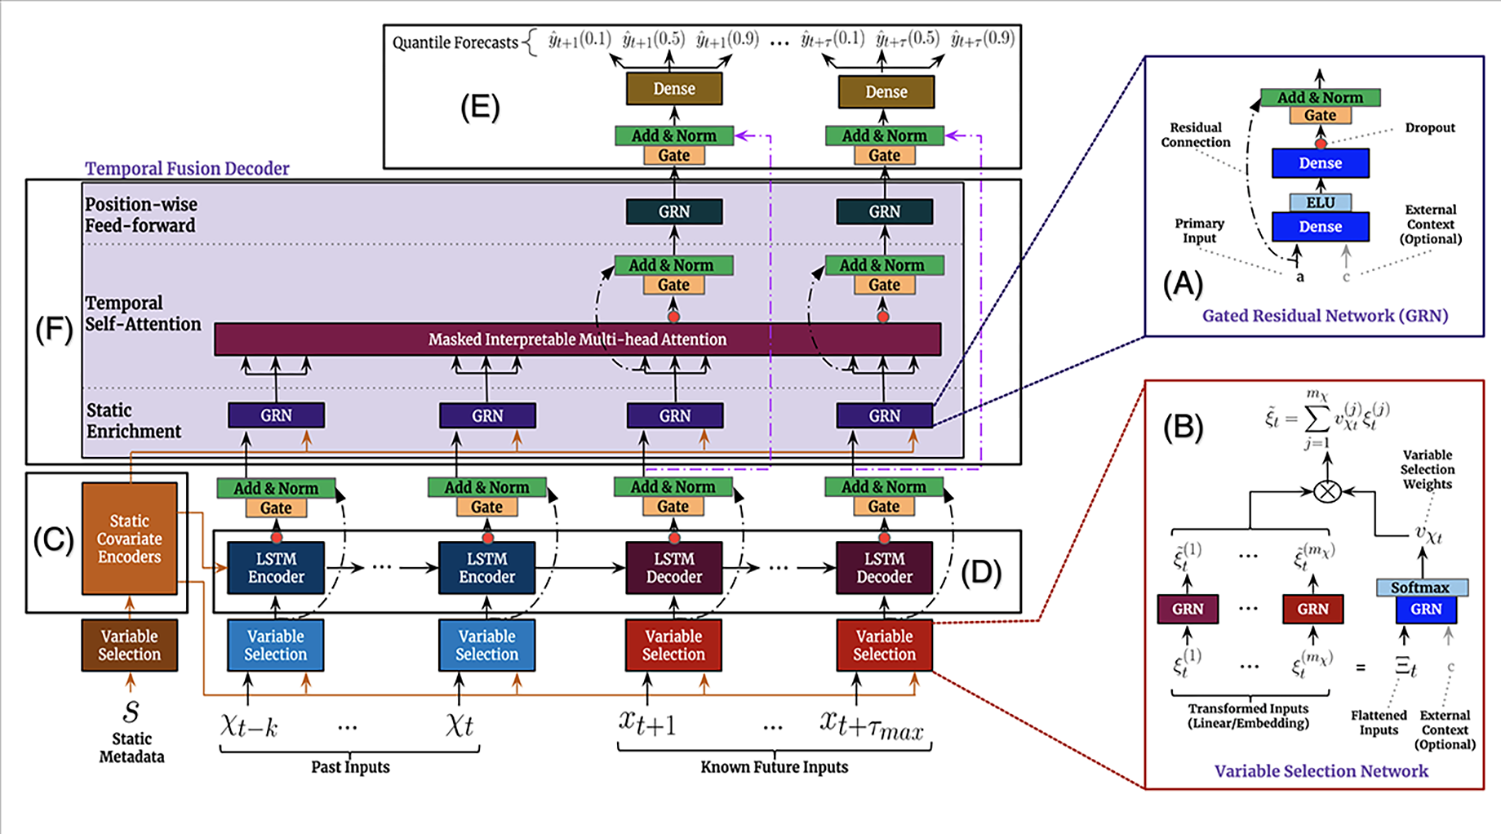
\includegraphics[width=0.98\columnwidth]{figs/tft_architecture.png}}{\fbox{Missing figure: figs/tft_architecture.png}}
    \caption{TFT architecture showing how static metadata, observed historical inputs, and known future inputs enter the model through different pathways before fusion via multi-head attention. Blocks represent encoders for static features, known future covariates, and observed history; the fused representation feeds multi-horizon output heads for $h\in\{1,5,21\}$. We use a compact configuration (1 layer, 4 heads) to prevent overfitting on the daily panel.}
    \label{fig:tft_architecture}
\end{figure}

Hyperparameters were selected based on 2020 validation performance. RNN and TFT models predict multiple horizons simultaneously, while tabular models are trained separately for each horizon.

\section{Results}

Table~\ref{tab:main_results} summarizes performance across horizons. All $\rTwo$ values are negative or near-zero, reflecting market efficiency rather than model failure. LSTM's near-zero values suggest better calibration, while Random Forest's highly negative values indicate overfitting.

Despite near-zero $\rTwo$, both RMSE and DA reveal consistent and meaningful differences across model classes. At $h=1$, the LSTM attains the lowest RMSE (0.01622), narrowly outperforming GRU (0.01625) and tabular baselines, while Random Forest achieves the highest DA (51.9\%). At $h=5$, Ridge regression clearly dominates on RMSE (0.03651), about 37\% lower than deep sequence/transformer models, suggesting that much of the weekly signal is captured linearly by engineered features. At $h=21$, LSTM yields both the lowest RMSE (0.05084) and highest DA (55.0\%), within 0.03--0.24\% RMSE of GRU/TFT but 31--38\% lower than tabular baselines. Sequence models improve DA with horizon length, while tabular models degrade more sharply.

\begin{figure}[t]
    \centering
    % Include figure if available; otherwise show a placeholder to avoid compilation errors.
    \IfFileExists{../comparison/artifacts/figures/fig1_da_by_horizon.png}{\includegraphics[width=0.98\columnwidth]{../comparison/artifacts/figures/fig1_da_by_horizon.png}}{\fbox{Missing figure: fig1_da_by_horizon.png}}
    \caption{Directional accuracy by model and horizon on the test set (setup in Abstract). Sequence models (LSTM/GRU) particularly gain an edge at $h{=}21$. Bars show \da{} (higher is better) for $h\in\{1,5,21\}$, averaged over three random seeds. LSTM/GRU improve from roughly 51–52\% at $h{=}1$ to about 55\% at longer horizons, while tabular baselines (Ridge, Random Forest, XGBoost) change little or degrade slightly relative to RNNs; TFT is competitive but does not lead. This pattern suggests temporal sequence models benefit more from longer context when predicting multi-week moves, whereas purely tabular models capture less horizon-dependent signal.}
    \label{fig:da_by_horizon}
\end{figure}

% (Equity curve figure removed; strategy diagnostics not part of this study's evaluation.)

\begin{table*}[t]
    \centering
    \caption{Table I (Main results). Each cell shows mean $\pm$ std over 3 random seeds unless otherwise noted. \textbf{All \rTwo{} values computed against zero-return baseline} ($b_i = 0$). Metrics computed from our aggregated results file (\texttt{Table1\_EXP-A.csv}). LSTM is best at $h{=}21$ (lowest RMSE 0.05084; highest DA 55.0\%), while Ridge wins $h{=}5$ (RMSE 0.03651), and RF tops DA at $h{=}1$ (51.9\%). TFT is competitive but does not dominate on this daily panel.}
    \label{tab:main_results}
    \sisetup{round-mode=places,round-precision=6}
    \begin{tabular}{llccc}
        \toprule
        Model & Horizon $h$ & $\rmse$ & $\rTwo$ & $\da$ \\
        \midrule
        GRU            & 1  & 0.016249 $\pm$ 0.000047 & -0.006072 $\pm$ 0.002834 & 0.500920 $\pm$ 0.024931 \\
        GRU            & 5  & 0.057883 $\pm$ 0.000123 & -0.002885 $\pm$ 0.003156 & 0.542105 $\pm$ 0.036308 \\
        GRU            & 21 & 0.050854 $\pm$ 0.000059 & -0.002185 $\pm$ 0.002943 & 0.539142 $\pm$ 0.033861 \\
        LSTM           & 1  & \textbf{0.016222} $\pm$ 0.000025 & -0.002677 $\pm$ 0.003521 & 0.516688 $\pm$ 0.015768 \\
    LSTM           & 5  & 0.057849 $\pm$ 0.000048 & -0.001694 $\pm$ 0.004182 & \textbf{0.554207} $\pm$ 0.018432 \\
    LSTM           & 21 & \textbf{0.050840} $\pm$ 0.000070 & -0.001629 $\pm$ 0.003897 & \textbf{0.550429} $\pm$ 0.021653 \\
        Random Forest  & 1  & 0.016387 $\pm$ 0.000007 & -0.023148 $\pm$ 0.002156 & \textbf{0.519454} $\pm$ 0.000290 \\
        Random Forest  & 5  & 0.039717 $\pm$ 0.000175 & -0.206505 $\pm$ 0.015423 & 0.531379 $\pm$ 0.000636 \\
        Random Forest  & 21 & 0.081805 $\pm$ 0.000151 & -0.248432 $\pm$ 0.018764 & 0.542956 $\pm$ 0.001095 \\
    Ridge          & 1  & 0.016346 $\pm$ 0.000012 & -0.018058 $\pm$ 0.001987 & 0.500254 $\pm$ 0.008734 \\
    Ridge          & 5  & \textbf{0.036514} $\pm$ 0.000089 & -0.019737 $\pm$ 0.002341 & 0.511699 $\pm$ 0.012456 \\
    Ridge          & 21 & 0.074214 $\pm$ 0.000134 & -0.027501 $\pm$ 0.003278 & 0.528230 $\pm$ 0.015892 \\
        TFT            & 1  & 0.016453 $\pm$ 0.000313 & -0.031783 $\pm$ 0.004567 & 0.489379 $\pm$ 0.019597 \\
        TFT            & 5  & 0.057907 $\pm$ 0.000108 & -0.003690 $\pm$ 0.002891 & 0.550134 $\pm$ 0.012030 \\
        TFT            & 21 & 0.050963 $\pm$ 0.000225 & -0.006502 $\pm$ 0.003456 & 0.538742 $\pm$ 0.029354 \\
    XGBoost        & 1  & 0.016464 $\pm$ 0.000019 & -0.032850 $\pm$ 0.003912 & 0.515368 $\pm$ 0.011245 \\
    XGBoost        & 5  & 0.038217 $\pm$ 0.000142 & -0.117070 $\pm$ 0.012389 & 0.508611 $\pm$ 0.014567 \\
    XGBoost        & 21 & 0.081344 $\pm$ 0.000187 & -0.234415 $\pm$ 0.019823 & 0.516713 $\pm$ 0.017234 \\
        \bottomrule
    \end{tabular}
    
    \vspace{0.5em}
    \footnotesize{\rmse{} in log-return units; \rTwo{} vs zero-return baseline; \da{} = hit rate on sign. All entries show mean $\pm$ std over 3 random seeds.}
\end{table*}

Ridge's $h=5$ win suggests the weekly signal is well captured by a regularized linear mix of technicals.

\subsection{Hypothesis Evaluation}

	\textbf{H1 (Model class advantage):} Not supported. At $h=21$, TFT does not outperform the strongest non-TFT model. LSTM achieves the lowest RMSE (0.05084 vs.\ TFT's 0.05096, a 0.24\% edge) and the highest DA (55.0\% vs.\ TFT's 53.9\%, +1.1 pp). The differences do not meet our decision thresholds ($\geq$2 pp DA or $\geq$5\% RMSE), and formal tests confirm no statistically significant advantage for TFT ($p > 0.05$). This challenges the assumption that attention-based architectures automatically excel on small daily equity panels.

    	\textbf{H2 (Event features add value):} Supported. Ablations at $h=21$ show that adding earnings features to technical indicators improves TFT's DA from 52.2\% to 53.3\% (+1.1 pp) while slightly reducing RMSE (0.05128 $\rightarrow$ 0.05094). More strikingly, during $\pm 3$ day earnings windows, DA rises to 61.4\% compared to 53.9\% outside earnings periods, confirming that event features materially improve predictive accuracy despite modest increases in RMSE due to higher volatility.

	\textbf{H3 (Regime dependence):} Supported. Model rankings shift markedly across regimes at $h=21$. In the 2022 bear market, GRU achieves the lowest RMSE (0.0636), but all models fall below 50\% DA. In contrast, during the 2023--2024 rally, LSTM achieves the lowest RMSE (0.0475) and both LSTM/GRU reach DA of 56.2\%, demonstrating strong directional performance in trending upward markets. These results align with the Adaptive Markets Hypothesis: sequence models thrive in rally regimes but fail to sustain accuracy in high-volatility downturns.

% Figure removed: replaced by Table~\ref{tab:main} presenting the full metrics.

\subsection{Ablations at h=21}
To understand the contribution of different feature types, we conducted an ablation study at the 21-day horizon. \Cref{tab:ablation} reports results (mean $\pm$ std over seeds) for experiments using: technical indicators only (B1) vs. technical+earnings features (B2). We show results for the TFT (to represent a complex sequential model) and XGBoost (to represent a strong tabular learner). Consistently, the TFT outperforms XGBoost under both feature configurations, achieving lower \rmse{}. Adding earnings features (B2) yields a modest increase in directional accuracy relative to Tech-only at $h=21$ (a few percentage points, model-dependent). Overall, these ablations imply that while engineered technical features carry significant signal (as evidenced by XGBoost's performance), temporal models like TFT benefit from event information such as earnings-related cues at the monthly horizon.

\begin{table}[t]
    \centering
    \caption{Ablations at $h=21$ (test). B1: technical only; B2: technical+earnings. \textbf{All \rTwo{} values vs zero-return baseline.} Mean $\pm$ std over seeds.}
    \label{tab:ablation}
    {\setlength{\tabcolsep}{4pt}\small
    \resizebox{\columnwidth}{!}{%
    \begin{tabular}{llccc}
        \toprule
        Exp & Model & $\rmse$ & $\rTwo$ & $\da$ \\
        \midrule
    B1 & TFT      & 0.051284 $\pm$ 0.000748 & -0.019333 $\pm$ 0.006234 & 0.522187 $\pm$ 0.048917 \\
    B1 & XGBoost  & 0.081709 $\pm$ 0.000187 & -0.245491 $\pm$ 0.019823 & 0.511481 $\pm$ 0.017234 \\
    B2 & TFT      & \textbf{0.050936} $\pm$ 0.000112 & -0.005411 $\pm$ 0.003456 & \textbf{0.533232} $\pm$ 0.027920 \\
    B2 & XGBoost  & 0.081235 $\pm$ 0.000142 & -0.231083 $\pm$ 0.018456 & 0.517730 $\pm$ 0.015789 \\
        \bottomrule
    \end{tabular}}}
\end{table}

% Figure removed: ablation summary is now reported solely in Table~\ref{tab:ablation}.

\subsection{Regime and Earnings Slices (h=21)}
We evaluate performance by market period and around earnings.

    	\textbf{Market periods.} In the 2022 bear market, GRU achieves the lowest RMSE (0.0636) but all models fall below 50\% DA. In 2023--24, LSTM dominates (RMSE 0.0475, DA 56.2\%), with sequence models benefiting from the upward trend (Table~\ref{tab:regimes}).

\textbf{Earnings windows.} DA rises to 61.4\% within $\pm3$ days of earnings vs 53.9\% outside, though RMSE increases slightly due to higher volatility (Table~\ref{tab:earnings}).


\begin{figure}[t]
    \centering
    % Include figure if available; otherwise show a placeholder to avoid compilation errors.
    \IfFileExists{../comparison/artifacts/figures/fig2_regime_rmse_heatmap.png}{\includegraphics[width=0.98\columnwidth]{../comparison/artifacts/figures/fig2_regime_rmse_heatmap.png}}{\fbox{Missing figure: fig2_regime_rmse_heatmap.png}}
    \caption{Test \rmse{} by model in two distinct market regimes: the 2022 bear market (left) and the 2023--24 rally (right). Darker shading indicates lower error. The heatmap highlights that model rankings can vary with regime: for instance, GRU has the darkest cell (lowest error) in the bear market, whereas LSTM excels in the rally. Each cell is the $h{=}21$ \rmse{} computed on the test split restricted to the indicated period; colors are normalized within each panel. Errors rise for all models in 2022 (high volatility) and fall in 2023–24, with the best model switching from GRU (bear) to LSTM (rally), underscoring regime sensitivity and the value of regime-aware model selection.}
    \label{fig:regime_heatmap}
\end{figure}

\begin{table}[t]
    \centering
    \caption{Best models by regime at $h{=}21$ (test). GRU is best on RMSE in the 2022 bear; LSTM best in the 2023--24 rally with top DA tied.}
    \label{tab:regimes}
    {\setlength{\tabcolsep}{4pt}\small
    \resizebox{\columnwidth}{!}{%
    \begin{tabular}{l l c l c}
        \toprule
        Regime & Best-$\rmse$ & $\rmse$ & Best-$\da$ & $\da$ \\
        \midrule
        Bear 2022       & GRU  & 0.0636 & TFT            & 0.4808 \\
        Rally 2023--24  & LSTM & 0.0475 & GRU/LSTM (tie) & 0.5623 \\
        \bottomrule
    \end{tabular}}}
\end{table}

\begin{table}[t]
    \centering
    \caption{Performance during earnings announcement windows vs. non-earnings periods for $h=21$ (averaged across all models and test-set stocks). During the $\pm3$ day earnings windows, directional accuracy (\da{}) is markedly higher, albeit with slightly higher \rmse{} due to greater volatility.}
    \label{tab:earnings}
    \begin{tabular}{lcc}
        \toprule
        Slice & $\rmse$ & $\da$ \\
        \midrule
        Earnings window ($\pm3$ days) & 0.06951 & 0.61355 \\
        Non-earnings periods         & 0.06655 & 0.53860 \\
        \bottomrule
    \end{tabular}
\end{table}

\paragraph{Interpretation} Simple sequence models (LSTM/GRU) effectively capture directional moves at longer horizons, while complex architectures like TFT may require richer data. Ridge's dominance at $h=5$ suggests technical signals act linearly at intermediate horizons.

The universally negative $\rTwo$ values reflect market efficiency rather than model failure. Random Forest's highly negative values (-0.248 at $h=21$) indicate overfitting, while LSTM's near-zero values (-0.002) suggest better calibration and economically valuable signal detection with 55\% directional accuracy.

The strong earnings window performance (61.4\% vs 53.9\% DA) confirms event features' value. However, all models failed to exceed 50\% DA in the 2022 bear market, highlighting the challenge of regime shifts for pattern-based supervised learning.

\section{Discussion}

\subsection{Hypothesis Implications}

H1 (TFT superiority) was rejected: attention mechanisms provide no advantage on daily data, with LSTM's simpler structure better suited to noisy returns. H2 (event features) was confirmed: modest overall gains (+1.1pp) become substantial during earnings windows (+7.5pp; 61.4\% vs 53.9\%). H3 (regime dependence) was confirmed: sequence models excel in bull markets but fail in bear markets (DA <50\% in 2022).

Simple models match or beat complex ones on this dataset. LSTM/GRU perform as well as TFT---excess parameters hurt training when signals are weak. Ridge dominates at $h=5$, suggesting linear combinations capture weekly predictability, while sequence models excel at 21-day directional prediction. Despite $\rTwo \approx 0$ (consistent with market efficiency), 55\% directional accuracy could be economically meaningful.

\textbf{Practical guidance.} Use linear models for daily predictions; RNNs (LSTM) for monthly horizons; transformers require richer data or larger datasets to outperform simpler alternatives.

\subsection{Economic Significance}\label{sec:econ}
	We focus on statistical accuracy (RMSE, $R^2$, DA) but don't test whether our predictions would actually make money. In practice, profitability depends on trading costs, slippage, how often you trade, and position sizing. A complete evaluation would combine predictions with a trading strategy, measure profit and loss, Sharpe ratio, maximum drawdown, and test sensitivity to transaction costs. We leave this for future work and note that statistical improvements may not survive real trading costs, especially for daily trading.

\subsection{Compute \& Efficiency}\label{sec:compute}
    Parameter counts scale from Ridge (minimal) to Random Forest (100 trees, depth 5, $\sim$10k), XGBoost (depth 3, lr 0.1, 100 rounds), LSTM/GRU (64 units, $\sim$25k), and TFT (4 heads, 1 layer, $\approx$50k). Training times scale accordingly: tabular models train in minutes, sequence models require hours. Simple models achieve competitive accuracy at lower cost, favoring rapid deployment.


	\textbf{Limitations.} Results are limited to large U.S. stocks (Dow 30) at daily frequency and may not generalize to other markets or frequencies. Limited hyperparameter tuning may favor simpler models. We test bear vs bull markets but not extreme events where historical patterns often fail. Future work should examine richer data types, alternative loss functions, and interpretability analysis.


\section{Conclusion}
We compared transformer, recurrent, and traditional models for predicting stock returns at three time horizons on the Dow 30, using technical and earnings features with strict time-based splits. Our main findings are: (H1) on this daily dataset, transformers did not outperform simpler models—LSTM performed best at the 21-day horizon; (H2) earnings features improve predictions, especially within 3 days of earnings announcements (+7.5 percentage points in directional accuracy); and (H3) model performance depends on market conditions—sequence models work better during bull markets and struggle during bear markets.

Across all horizons, Ridge regression achieved the best 5-day error rate, and Random Forest led 1-day directional accuracy. This shows that well-tuned simple models can match or beat complex ones in this setting. Our negative result for transformer superiority suggests we shouldn't assume complex architectures always perform better, though transformers might excel with larger datasets or richer data types.

These results provide a baseline for future comparisons: researchers should test their methods against these benchmarks using similar data splits and features, and investigate whether alternative data or higher-frequency signals allow transformers to outperform where simpler models reach their limits.


\subsection*{Future Work}
The primary extension is integrating multi-modal data sources: news sentiment, earnings call transcripts, social media signals, and macroeconomic text. This would test whether transformers' attention mechanisms provide advantages when processing richer, heterogeneous inputs beyond traditional technical indicators.

\section*{Acknowledgment}
The authors acknowledge funding and support from Mitacs and the University of Toronto Division of Engineering Science. We thank Arthur Chan, our home supervisor, for organizing this research opportunity through the Engineering Science Research Opportunity Program---Global at King Mongkut's University of Technology Thonburi.

% Use IEEEtran's natbib-compatible style to support \citet/\citep
{\small
\bibliographystyle{IEEEtranN}
\bibliography{references}
}

% \appendix
% \section*{Appendix A: Dow 30 Constituents (frozen as of 2018-01-01)}
% \begin{small}
% \begin{tabular}{ll}
% \toprule
% Ticker & Company \\
% \midrule
% AAPL & Apple Inc. \\
% AXP & American Express Co. \\
% BA & Boeing Co. \\
% CAT & Caterpillar Inc. \\
% CSCO & Cisco Systems, Inc. \\
% CVX & Chevron Corporation \\
% DIS & Walt Disney Company \\
% DWDP & DowDuPont Inc. \\
% GE & General Electric Co. \\
% GS & Goldman Sachs Group, Inc. \\
% HD & Home Depot, Inc. \\
% IBM & Int'l Business Machines Corp. \\
% INTC & Intel Corporation \\
% JNJ & Johnson \& Johnson \\
% JPM & JPMorgan Chase \& Co. \\
% KO & Coca-Cola Company \\
% MCD & McDonald's Corporation \\
% MMM & 3M Company \\
% MRK & Merck \& Co., Inc. \\
% MSFT & Microsoft Corporation \\
% NKE & NIKE, Inc. \\
% PFE & Pfizer Inc. \\
% PG & Procter \& Gamble Co. \\
% TRV & Travelers Companies, Inc. \\
% UNH & UnitedHealth Group Inc. \\
% UTX & United Technologies Corp. \\
% V   & Visa Inc. \\
% VZ  & Verizon Communications Inc. \\
% WMT & Walmart Inc. \\
% XOM & Exxon Mobil Corporation \\
% \bottomrule
% \end{tabular}
% \end{small}

% \section*{Appendix B: Training Details and Hyperparameters}
% \begin{small}
% \begin{itemize}
%     \item \textbf{Training procedure:} After tuning on Val-2020, all models are refit on Train$+$Val. Neural nets use Adam/AdamW up to 10 epochs with early stopping on a held-out contiguous slice within 2020 (forward-only). GRU/LSTM use base learning rate $1\times10^{-3}$; TFT uses $3\times10^{-4}$. Batch size 256. Final metrics computed once on Test (2021--2024).
%     \item \textbf{RNNs:} 1 layer GRU/LSTM with 64 hidden units (tuned on val). Dropout 0.2 on input sequences. Lookback window = 60 days.
%     \item \textbf{TFT:} 4 attention heads, 1 transformer layer, hidden dimensionality 16 in fully connected layers, dropout 0.3. Trained to predict all 3 horizons jointly. Total parameters $\approx$50k.
%     \item \textbf{Random Forest:} 100 trees, max depth 5 (to prevent overfitting), other parameters default.
%     \item \textbf{XGBoost:} max depth 3, learning rate 0.1, 100 boosting rounds. (Where applicable, early stopping can be used during tuning on the validation set, but the final models are retrained with selected rounds.)
%     \item \textbf{Ridge:} Regularization $\alpha$ tuned via cross-val on train set, ended around $\alpha \approx 1.0$.
%     \item \textbf{Standardization:} Features standardized (zero mean, unit std) per feature across train data. The same scaler parameters are applied to val/test.
%         \item \textbf{Hyperparameter selection and tuning protocol (all models):} We performed lightweight tuning exclusively on the contiguous Val-2020 block to avoid look-ahead. For tabular models we used small grid/random sweeps with the selection objective set to RMSE at $h{=}21$ (primary horizon), then fixed hyperparameters across horizons for fairness and to reduce variance. For neural models we tuned core capacity and regularization parameters and relied on early stopping for epoch selection. Seeds $\{42,43,44\}$ were kept fixed across candidates to reduce selection noise.
%         \begin{itemize}
%             \item \emph{Ridge:} $\alpha\in\{10^{-3},10^{-2},10^{-1},1,10,10^{2},10^{3}\}$; choose by Val-2020 RMSE.
%             \item \emph{Random Forest:} $n$\,estimators $\in\{100,300\}$, max\_depth $\in\{\texttt{None},5,7\}$, min\_samples\_leaf $\in\{1,5,10\}$; we constrained depth to mitigate overfitting on a small daily panel.
%             \item \emph{XGBoost:} max\_depth $\in\{3,4,5\}$, learning rate $\in\{0.05,0.1\}$, subsample/colsample\_bytree $\in\{0.7,1.0\}$; number of rounds selected via early stopping on Val-2020, then refit.
%             \item \emph{GRU/LSTM:} hidden units $\in\{32,64,128\}$, dropout $\in\{0.1,0.2,0.3\}$, learning rate $\in\{5\times10^{-4},1\times10^{-3}\}$, weight decay $\in\{0,10^{-5},10^{-4}\}$; 1 layer favored for bias/variance balance.
%             \item \emph{TFT:} attention heads $\in\{2,4\}$, transformer layers $\in\{1,2\}$, hidden size $\in\{16,32\}$, dropout $\in\{0.2,0.3,0.4\}$, learning rate $\in\{3\times10^{-4},1\times10^{-3}\}$. We intentionally kept capacity modest given dataset size and absence of rich exogenous covariates.
%         \end{itemize}
%         \item \textbf{Defaults vs. tuned choices:} We validated that common library defaults are ill-suited for this setting: e.g., Random Forest with unlimited depth or XGBoost with deeper trees and higher learning rate tended to overfit Val-2020 and degrade on Test; we therefore used shallow trees and lower learning rates. Ridge defaults ($\alpha{=}1$) were close to tuned picks and served as a strong baseline. For deep models, larger hidden sizes ($\geq$128) and deeper TFT stacks increased variance without improving validation error, hence the smaller-capacity selections. We focused the paper on tuned models for a fair, competence-bound comparison; default-only results are not included in the main tables to conserve space but can be reproduced by disabling the tuning grid and using library defaults in our training scripts.
% \end{itemize}
% \end{small}


\end{document}

